% =============================================================================
% Equipo 8 - Tarea 3: Inteligencia Artificial en el Procesamiento de Imágenes
% Universidad Autónoma de Aguascalientes - ICI 7°A
% Compilar con LuaLaTeX:  python generar_macros.py && lualatex reporte_tarea6.tex (dos veces)
% =============================================================================
\documentclass[11pt,letterpaper]{article}

% ---------------- Enlace al repositorio (EDITAR ESTA LÍNEA) ------------------
\newcommand{\Repositorio}{\textcolor{red}{[pegar aquí el enlace del repositorio de GitHub]}}
% Ejemplo: \newcommand{\Repositorio}{\url{https://github.com/usuario/tarea6-cnn-mnist}}

% ---------------- Idioma y tipografía ----------------------------------------
% Español mediante el archivo .ini de babel. Esta instalación no incluye patrones de
% guionado para español; se desactiva el guionado para evitar cortes incorrectos.
\usepackage{babel}
\babelprovide[import,main,hyphenrules=nohyphenation]{spanish}
\usepackage{mathpazo}
\usepackage[no-math]{fontspec}
\setmainfont{TeX Gyre Pagella}
\setsansfont{TeX Gyre Heros}[Scale=MatchLowercase]
\setmonofont{Latin Modern Mono}
\usepackage{amsmath,amssymb}
\usepackage{microtype}
\emergencystretch=2.5em
\linespread{1.08}

% ---------------- Página -----------------------------------------------------
\usepackage[letterpaper,top=2.5cm,bottom=2.5cm,left=2.5cm,right=2.5cm,headheight=14pt]{geometry}
\usepackage{fancyhdr}
\usepackage{titlesec}
\usepackage{enumitem}
\setlist{itemsep=2pt,topsep=4pt}
\setlength{\parskip}{4pt}

% ---------------- Tablas, figuras, color --------------------------------------
\usepackage{graphicx}
\graphicspath{{../figuras/}}
\usepackage{booktabs,tabularx,array,multirow,makecell}
\usepackage[table]{xcolor}
\usepackage{caption}
\captionsetup{font=small,labelfont=bf,labelsep=period,margin=0.5cm}
\usepackage{float}
\usepackage{tikz}
\usetikzlibrary{positioning,arrows.meta,calc,decorations.pathreplacing}
\usepackage{listings}
\usepackage{tcolorbox}

\definecolor{azul}{HTML}{2A78D6}
\definecolor{azulclaro}{HTML}{E3EEFB}
\definecolor{naranja}{HTML}{EB6834}
\definecolor{naranjaclaro}{HTML}{FCE8DF}
\definecolor{gris}{HTML}{52514E}
\definecolor{grisclaro}{HTML}{F3F3F1}

\usepackage[hidelinks]{hyperref}
\usepackage{xurl}

% Nombres en español de México
\setlocalecaption{spanish}{table}{Tabla}
\setlocalecaption{spanish}{listtable}{Índice de tablas}
\setlocalecaption{spanish}{contents}{Índice}
\setlocalecaption{spanish}{references}{Referencias}

% Títulos de sección
\titleformat{\section}{\Large\bfseries\color{azul!70!black}}{\thesection.}{0.6em}{}
\titleformat{\subsection}{\large\bfseries}{\thesubsection}{0.6em}{}
\titleformat{\subsubsection}{\normalsize\bfseries}{\thesubsubsection}{0.6em}{}
\titlespacing*{\section}{0pt}{14pt}{6pt}
\titlespacing*{\subsection}{0pt}{10pt}{4pt}

% Encabezado y pie (sin fecha)
\pagestyle{fancy}
\fancyhf{}
\fancyhead[L]{\small\color{gris}Procesamiento de Imágenes}
\fancyhead[R]{\small\color{gris}Equipo 8 - Tarea 3: IA en el procesamiento de imágenes}
\fancyfoot[C]{\small\thepage}
\renewcommand{\headrulewidth}{0.4pt}

% Código
\lstset{
  basicstyle=\ttfamily\footnotesize,
  keywordstyle=\color{azul!80!black},
  commentstyle=\color{gris}\itshape,
  stringstyle=\color{naranja!80!black},
  backgroundcolor=\color{grisclaro},
  frame=single, rulecolor=\color{black!15},
  breaklines=true, columns=fullflexible, keepspaces=true,
  showstringspaces=false, xleftmargin=4pt, xrightmargin=4pt,
  language=Python
}

% Pregunta destacada
\newtcolorbox{pregunta}{colback=azulclaro,colframe=azul,boxrule=0pt,leftrule=3pt,
  arc=0pt,left=6pt,right=6pt,top=4pt,bottom=4pt,fontupper=\itshape}

\newcommand{\pct}{\,\%}
% Archivo generado automáticamente por generar_macros.py - no editar a mano
\newcommand{\ParamTotal}{421{,}642}
\newcommand{\AccTrain}{99.82}
\newcommand{\AccVal}{99.18}
\newcommand{\AccTest}{99.37}
\newcommand{\ErrTest}{0.63}
\newcommand{\LossTrain}{0.0065}
\newcommand{\LossVal}{0.0334}
\newcommand{\LossTest}{0.0229}
\newcommand{\NErroresTest}{63}
\newcommand{\NAciertosTest}{9{,}937}
\newcommand{\Epocas}{10}
\newcommand{\TamLote}{128}
\newcommand{\TiempoEnt}{251}
\newcommand{\TiempoEntMin}{4.2}
\newcommand{\TiempoEpoca}{25.1}
\newcommand{\TiempoInf}{2.6}
\newcommand{\TiempoInfImg}{0.26}
\newcommand{\MacroP}{99.36}
\newcommand{\MacroR}{99.36}
\newcommand{\MacroF}{99.36}
\newcommand{\VersionTorch}{2.15.0}
\newcommand{\VersionPython}{3.13.18}
\newcommand{\FilasHistorial}{1 & 0.2729 & 91.71 & 0.0689 & 97.98 & 24.9 \\
2 & 0.0893 & 97.36 & 0.0483 & 98.68 & 23.0 \\
3 & 0.0639 & 98.08 & 0.0482 & 98.60 & 24.1 \\
4 & 0.0541 & 98.37 & 0.0427 & 98.76 & 24.5 \\
5 & 0.0446 & 98.70 & 0.0367 & 98.98 & 23.9 \\
6 & 0.0384 & 98.80 & 0.0371 & 98.80 & 25.7 \\
7 & 0.0333 & 98.98 & 0.0358 & 98.98 & 26.7 \\
8 & 0.0303 & 99.05 & 0.0414 & 98.96 & 26.9 \\
9 & 0.0262 & 99.13 & 0.0414 & 99.08 & 26.1 \\
10 & 0.0247 & 99.21 & 0.0334 & 99.18 & 25.3 \\}
\newcommand{\FilasPorClase}{0 & 99.59 & 99.69 & 99.64 & 980 \\
1 & 99.74 & 99.74 & 99.74 & 1{,}135 \\
2 & 99.71 & 99.22 & 99.47 & 1{,}032 \\
3 & 99.60 & 99.41 & 99.50 & 1{,}010 \\
4 & 99.09 & 99.80 & 99.44 & 982 \\
5 & 98.55 & 99.10 & 98.83 & 892 \\
6 & 99.69 & 99.58 & 99.63 & 958 \\
7 & 98.75 & 99.71 & 99.23 & 1{,}028 \\
8 & 99.18 & 99.18 & 99.18 & 974 \\
9 & 99.70 & 98.22 & 98.95 & 1{,}009 \\}
\newcommand{\PeorClase}{5}
\newcommand{\PeorClaseF}{98.83}
\newcommand{\PeorClaseR}{99.10}
\newcommand{\MejorClase}{1}
\newcommand{\MejorClaseF}{99.74}
\newcommand{\ErroresNueve}{18}
\newcommand{\ErroresCinco}{8}
\newcommand{\ErroresUno}{3}
\newcommand{\ErroresCero}{3}
\newcommand{\ParA}{9$\to$5}
\newcommand{\ParAN}{7}
\newcommand{\ParB}{2$\to$7}
\newcommand{\ParBN}{6}
\newcommand{\ParC}{9$\to$4}
\newcommand{\ParCN}{5}
\newcommand{\ParD}{9$\to$8}
\newcommand{\ParDN}{4}
\newcommand{\ParE}{5$\to$3}
\newcommand{\ParEN}{4}
\newcommand{\ErrAIdx}{9729}
\newcommand{\ErrAReal}{5}
\newcommand{\ErrAPred}{6}
\newcommand{\ErrAConf}{99.9}
\newcommand{\ErrBIdx}{1014}
\newcommand{\ErrBReal}{6}
\newcommand{\ErrBPred}{5}
\newcommand{\ErrBConf}{99.9}
\newcommand{\ErrCIdx}{2654}
\newcommand{\ErrCReal}{6}
\newcommand{\ErrCPred}{1}
\newcommand{\ErrCConf}{99.9}
\newcommand{\ErrDIdx}{4176}
\newcommand{\ErrDReal}{2}
\newcommand{\ErrDPred}{7}
\newcommand{\ErrDConf}{99.9}
\newcommand{\ErrEIdx}{4740}
\newcommand{\ErrEReal}{3}
\newcommand{\ErrEPred}{5}
\newcommand{\ErrEConf}{98.9}
\newcommand{\KnnAcc}{96.92}
\newcommand{\KnnPred}{10.6}
\newcommand{\KnnAjuste}{0.2}
\newcommand{\HogAcc}{97.23}
\newcommand{\HogAjuste}{49}
\newcommand{\HogExtr}{10}
\newcommand{\HogPred}{0.02}
\newcommand{\HogParam}{3{,}250}
\newcommand{\HogDim}{324}
\newcommand{\HogErrores}{277}
\newcommand{\KnnErrores}{308}


% ---------------- Citas en formato APA (autor, año) ---------------------------
\usepackage{etoolbox}
\makeatletter
\newcommand{\defcita}[3]{\csdef{citA@#1}{#2}\csdef{citY@#1}{#3}}
\newcommand{\cit@chk}[1]{\ifcsdef{citA@#1}{}{\PackageError{citas}{Cita no definida: #1}{}}}
\newcommand{\cit@item}[1]{\cit@chk{#1}\cit@sep\csuse{citA@#1}, \csuse{citY@#1}\gdef\cit@sep{; }}
\newcommand{\parencite}[1]{(\gdef\cit@sep{}\forcsvlist{\cit@item}{#1})}
\newcommand{\textcite}[1]{\cit@chk{#1}\csuse{citA@#1} (\csuse{citY@#1})}
\makeatother
\defcita{adam}{Kingma y Ba}{2015}
\defcita{cortes1995}{Cortes y Vapnik}{1995}
\defcita{cover1967}{Cover y Hart}{1967}
\defcita{dalal2005}{Dalal y Triggs}{2005}
\defcita{deng2009}{Deng et~al.}{2009}
\defcita{dosovitskiy2021}{Dosovitskiy et~al.}{2021}
\defcita{freeman1961}{Freeman}{1961}
\defcita{gonzalez2018}{Gonzalez y Woods}{2018}
\defcita{goodfellow}{Goodfellow et~al.}{2016}
\defcita{guo2017}{Guo et~al.}{2017}
\defcita{he2016}{He et~al.}{2016}
\defcita{ioffe2015}{Ioffe y Szegedy}{2015}
\defcita{lecun1998}{LeCun, Bottou, et~al.}{1998}
\defcita{lecun_mnist}{LeCun, Cortes, y Burges}{1998}
\defcita{lowe2004}{Lowe}{2004}
\defcita{nair2010}{Nair y Hinton}{2010}
\defcita{omahony2020}{O'Mahony et~al.}{2020}
\defcita{pan2010}{Pan y Yang}{2010}
\defcita{paszke2019}{Paszke et~al.}{2019}
\defcita{pedregosa2011}{Pedregosa et~al.}{2011}
\defcita{ronneberger2015}{Ronneberger et~al.}{2015}
\defcita{rosenblatt}{Rosenblatt}{1958}
\defcita{rumelhart}{Rumelhart et~al.}{1986}
\defcita{selvaraju2017}{Selvaraju et~al.}{2017}
\defcita{simard2003}{Simard et~al.}{2003}
\defcita{sokolova2009}{Sokolova y Lapalme}{2009}
\defcita{srivastava2014}{Srivastava et~al.}{2014}
\defcita{szeliski2022}{Szeliski}{2022}
\defcita{tan2019}{Tan y Le}{2019}
\defcita{vaswani2017}{Vaswani et~al.}{2017}
\defcita{yosinski2014}{Yosinski et~al.}{2014}

% =============================================================================
\begin{document}

% ---------------- PORTADA ----------------------------------------------------
\begin{titlepage}
  \thispagestyle{empty}
  \centering
  \vspace*{0.5cm}
  {\LARGE\bfseries Universidad Autónoma de Aguascalientes\par}
  \vspace{0.6cm}
  {\Large ICI 7°A\par}
  \vspace{3.2cm}
  {\color{azul}\rule{\linewidth}{1.2pt}}\par\vspace{0.5cm}
  {\large\scshape Equipo 8 - Tarea 3\par}\vspace{0.3cm}
  {\huge\bfseries Inteligencia Artificial en el\\[0.15cm] Procesamiento de Imágenes\par}
  \vspace{0.4cm}
  {\color{azul}\rule{\linewidth}{1.2pt}}\par
  \vspace{2.2cm}
  {\large
  \begin{tabular}{rl}
    \textbf{Materia:}  & Procesamiento de Imágenes \\[0.25cm]
    \textbf{Profesor:} & Hermilo Sánchez Cruz \\
  \end{tabular}\par}
  \vfill
  {\large\textbf{Alumnos:}\par}
  \vspace{0.3cm}
  {\large
  Hernández Herrera Rodrigo\\[0.15cm]
  Huizar Gael\\[0.15cm]
  Mata Araiza Maria Fernanda\par}
  \vspace*{1.5cm}
\end{titlepage}

% ---------------- ÍNDICE -----------------------------------------------------
\setcounter{page}{2}
\tableofcontents
\vspace{0.6cm}
\begin{tcolorbox}[colback=grisclaro,colframe=black!15,boxrule=0.4pt,arc=1pt,title={\bfseries Entregables},coltitle=black,colbacktitle=black!8]
\begin{itemize}[leftmargin=1.2em]
  \item \textbf{Reporte:} este documento (PDF).
  \item \textbf{Código fuente comentado:} \texttt{cnn\_mnist.py} (CNN en PyTorch) y \texttt{baseline\_clasico.py} (métodos clásicos de comparación), disponibles en el repositorio: \Repositorio.
  \item \textbf{Figuras y gráficas:} carpeta \texttt{figuras/} del repositorio (todas se reproducen en este reporte).
  \item \textbf{Resultados numéricos:} carpeta \texttt{resultados/} (métricas en JSON, historial de entrenamiento, pesos del modelo).
  \item \textbf{Bibliografía:} en formato APA, al final del documento.
\end{itemize}
\end{tcolorbox}

\section*{Objetivo}
\addcontentsline{toc}{section}{Objetivo}
Analizar y estudiar, en equipo, el papel de la Inteligencia Artificial (IA) en el procesamiento de imágenes, comprendiendo los fundamentos de las redes neuronales profundas y comparando su desempeño con los métodos clásicos de visión por computadora. El trabajo se divide en tres partes: una investigación bibliográfica (Parte~I), una comparación crítica entre métodos clásicos y aprendizaje profundo (Parte~II) y la implementación, entrenamiento y análisis de una red neuronal convolucional para clasificar los dígitos de MNIST (Parte~III).

\clearpage
% =============================================================================
\section{Parte I. Investigación bibliográfica}
% =============================================================================

\subsection{¿Qué es una red neuronal artificial y cuáles son sus componentes básicos?}

Una \textbf{red neuronal artificial} (RNA) es un modelo computacional, inspirado de forma muy simplificada en el sistema nervioso, que aprende una función $\hat{y} = f(\mathbf{x};\boldsymbol{\theta})$ que relaciona entradas con salidas ajustando sus parámetros $\boldsymbol{\theta}$ a partir de ejemplos, en lugar de programarse con reglas explícitas \parencite{goodfellow}. Su unidad básica es la \textbf{neurona artificial}, heredera del perceptrón de \textcite{rosenblatt}: calcula una suma ponderada de sus entradas, le añade un sesgo y aplica una función de activación no lineal:
\begin{equation}
  y = \varphi\Big(\sum_{i=1}^{n} w_i x_i + b\Big) = \varphi\left(\mathbf{w}^{\top}\mathbf{x} + b\right).
  \label{eq:neurona}
\end{equation}

Sus componentes básicos son:
\begin{itemize}
  \item \textbf{Entradas} ($\mathbf{x}$): los datos que recibe la red; en imágenes, las intensidades de los píxeles.
  \item \textbf{Pesos} ($\mathbf{w}$) \textbf{y sesgos} ($b$): los parámetros que se aprenden. Cada peso indica la importancia de una entrada; el sesgo desplaza el umbral a partir del cual la neurona se activa.
  \item \textbf{Función de activación} ($\varphi$): introduce no linealidad (sigmoide, tangente hiperbólica, ReLU). Sin ella, cualquier número de capas equivaldría a una sola transformación lineal.
  \item \textbf{Capas}: una capa de entrada, una o más capas ocultas y una capa de salida. En clasificación, la salida suele pasar por \emph{softmax} para obtener una probabilidad por clase. Una red con muchas capas ocultas es una red \emph{profunda}.
  \item \textbf{Función de pérdida} ($L$): mide qué tan lejos está la predicción de la etiqueta real (entropía cruzada para clasificación, error cuadrático medio para regresión).
  \item \textbf{Algoritmo de aprendizaje}: la \emph{retropropagación} \parencite{rumelhart} calcula, con la regla de la cadena, el gradiente de la pérdida respecto de cada parámetro, y un \emph{optimizador} (descenso de gradiente estocástico, Adam \parencite{adam}) actualiza los parámetros en dirección contraria al gradiente: $\boldsymbol{\theta} \leftarrow \boldsymbol{\theta} - \eta\,\nabla_{\boldsymbol{\theta}}L$, donde $\eta$ es la tasa de aprendizaje.
\end{itemize}

\subsection{Diferencia entre una red neuronal tradicional y una red neuronal convolucional (CNN)}

Una red neuronal \textbf{tradicional} (perceptrón multicapa, MLP) está formada por capas \emph{totalmente conectadas}: cada neurona recibe la salida de todas las neuronas de la capa anterior. Para procesar una imagen hay que aplanarla en un vector, con lo que se pierde la estructura espacial (qué píxeles son vecinos), y el número de parámetros crece con el tamaño de la imagen.

Una \textbf{red neuronal convolucional} \parencite{lecun1998} sustituye las capas densas iniciales por capas convolucionales, que aprovechan tres ideas:
\begin{enumerate}
  \item \textbf{Conectividad local}: cada neurona solo observa una pequeña región de la entrada (su \emph{campo receptivo}), porque en una imagen los píxeles relacionados están cerca unos de otros.
  \item \textbf{Pesos compartidos}: el mismo filtro (\emph{kernel}) se aplica en todas las posiciones de la imagen. Así, un patrón (por ejemplo, un borde diagonal) se detecta igual sin importar dónde aparezca (equivarianza a la traslación) y el número de parámetros no depende del tamaño de la imagen.
  \item \textbf{Jerarquía de rasgos}: las primeras capas detectan bordes y texturas simples; las intermedias, combinaciones de ellos (esquinas, curvas, partes); las profundas, objetos completos.
\end{enumerate}

Un ejemplo numérico muestra la diferencia. Para una imagen de MNIST ($28\times28 = 784$ píxeles), una capa densa de 128 neuronas necesita $784\cdot128 + 128 = 100{,}480$ parámetros, mientras que una capa convolucional de 32 filtros de $3\times3$ necesita $(3\cdot3\cdot1+1)\cdot32 = 320$ parámetros. Para una imagen a color de $224\times224$, la misma capa densa requeriría más de 19 millones de parámetros, mientras que la capa convolucional pasaría a $(3\cdot3\cdot3+1)\cdot32 = 896$. La Tabla~\ref{tab:mlp-cnn} resume las diferencias.

\begin{table}[H]
\centering
\caption{Red neuronal tradicional (MLP) frente a red neuronal convolucional (CNN).}
\label{tab:mlp-cnn}
\small
\begin{tabularx}{\linewidth}{>{\bfseries\raggedright\arraybackslash}p{2.6cm}>{\raggedright\arraybackslash}X>{\raggedright\arraybackslash}X}
\toprule
Aspecto & MLP (totalmente conectada) & CNN \\
\midrule
Conexiones & Cada neurona con todas las de la capa anterior & Locales (campo receptivo pequeño) \\
Entrada & Vector aplanado; se pierde la estructura 2D & Tensor (canales $\times$ alto $\times$ ancho); conserva la estructura espacial \\
Parámetros & Crecen con el tamaño de la imagen & Dependen del tamaño y número de filtros, no de la imagen \\
Traslaciones & Un mismo patrón en otra posición es una entrada distinta & Equivarianza a traslaciones por pesos compartidos (e invariancia parcial gracias al \emph{pooling}) \\
Rasgos & Debe aprenderlos sin estructura previa o recibirlos ya diseñados & Aprende una jerarquía de filtros directamente de los píxeles \\
Uso típico & Datos tabulares, vectores de rasgos & Imágenes, video, señales con estructura espacial o temporal \\
\bottomrule
\end{tabularx}
\end{table}

\subsection{Propósito de las capas convolucionales, las funciones de activación y las capas de agrupamiento}

\paragraph{Capas convolucionales.} Aplican $K$ filtros aprendibles que se deslizan sobre la entrada; cada filtro produce un \emph{mapa de activación} que indica en qué posiciones aparece el patrón que el filtro detecta. Para una entrada $I$ y un filtro $K$ de tamaño $k\times k$:
\begin{equation}
  S(i,j) = \sum_{m=0}^{k-1}\sum_{n=0}^{k-1} I(i+m,\,j+n)\,K(m,n) + b .
\end{equation}
(Estrictamente es una correlación cruzada, que es lo que implementan las bibliotecas.) Es la misma operación de filtrado espacial que se usa en el procesamiento clásico, por ejemplo con los filtros de Sobel, Laplaciano o Gaussiano \parencite{gonzalez2018}, con la diferencia de que los coeficientes no se diseñan a mano, sino que se aprenden. El tamaño espacial de la salida es $O = (W - k + 2P)/S + 1$, donde $W$ es el tamaño de la entrada, $P$ el relleno (\emph{padding}) y $S$ el paso (\emph{stride}). En la red de la Parte~III, con $W=28$, $k=3$, $P=1$ y $S=1$, se obtiene $O=28$: la convolución conserva el tamaño.

\paragraph{Funciones de activación.} Introducen no linealidad, lo que permite a la red aproximar funciones complejas. La más usada en capas ocultas es \textbf{ReLU}, $f(x)=\max(0,x)$ \parencite{nair2010}: es barata de calcular, no se satura para valores positivos (evita el desvanecimiento del gradiente típico de la sigmoide y la tangente hiperbólica) y produce activaciones dispersas. En la capa de salida, \textbf{softmax} convierte las puntuaciones (\emph{logits}) en probabilidades: $\operatorname{softmax}(\mathbf{z})_k = e^{z_k}/\sum_j e^{z_j}$.

\paragraph{Capas de agrupamiento (\emph{pooling}).} Reducen la resolución espacial de los mapas de activación. El \emph{max pooling} de $2\times2$ con paso 2 conserva el valor máximo de cada bloque y reduce a la cuarta parte el número de activaciones. Con ello: (i) disminuyen el cómputo y los parámetros de las capas posteriores; (ii) crece el campo receptivo de las capas siguientes, que ven regiones más amplias de la imagen original, y (iii) la red gana cierta invariancia a pequeñas traslaciones y deformaciones. También existen el \emph{average pooling} y el \emph{global average pooling}, este último muy usado al final de arquitecturas modernas como ResNet.

\subsection{Arquitecturas ResNet, EfficientNet, U-Net y Vision Transformer}

\paragraph{ResNet.} \textcite{he2016} observaron que, al apilar más capas, la exactitud se satura y después empeora \emph{incluso en entrenamiento}; a esto lo llamaron problema de \emph{degradación}, y no se debe al sobreajuste. Su solución fue el \textbf{bloque residual}: en lugar de pedir a un grupo de capas que aprenda directamente una transformación $H(\mathbf{x})$, se le pide que aprenda el residuo $F(\mathbf{x}) = H(\mathbf{x}) - \mathbf{x}$, y la salida se obtiene con una conexión de atajo (\emph{skip connection}) identidad:
\begin{equation}
  \mathbf{y} = F(\mathbf{x}, \{W_i\}) + \mathbf{x}.
\end{equation}
Si la identidad es la mejor opción, basta con llevar $F$ a cero, lo cual es fácil de aprender, y el gradiente fluye sin obstáculos por los atajos. Esto permitió entrenar redes de 50, 101 y 152 capas (y más de 1000 en CIFAR-10), con bloques \emph{bottleneck} ($1\times1$, $3\times3$, $1\times1$) y normalización por lotes \parencite{ioffe2015}. Un conjunto de ResNets ganó la competencia ILSVRC~2015 de clasificación con 3.57\pct{} de error \emph{top-5}.

\paragraph{EfficientNet.} \textcite{tan2019} estudiaron cómo \emph{escalar} una CNN cuando se dispone de más recursos. En lugar de aumentar de forma arbitraria solo la profundidad (número de capas), la anchura (número de canales) o la resolución de entrada, propusieron el \textbf{escalado compuesto}, que aumenta las tres dimensiones de manera balanceada con un solo coeficiente $\phi$:
\begin{equation}
  d = \alpha^{\phi},\qquad w = \beta^{\phi},\qquad r = \gamma^{\phi},\qquad \text{con } \alpha\cdot\beta^{2}\cdot\gamma^{2}\approx 2,
\end{equation}
de modo que cada incremento unitario de $\phi$ aproximadamente duplica las operaciones (FLOPs). La red base, EfficientNet-B0, se obtuvo con búsqueda automática de arquitecturas (NAS) y usa bloques MBConv (convoluciones invertidas con \emph{squeeze-and-excitation}). Escalándola se obtiene la familia B0--B7; EfficientNet-B7 alcanzó alrededor de 84\pct{} de exactitud \emph{top-1} en ImageNet siendo 8.4 veces más pequeña y 6.1 veces más rápida en inferencia que la mejor CNN anterior.

\paragraph{U-Net.} \textcite{ronneberger2015} la propusieron para la \textbf{segmentación} de imágenes biomédicas, es decir, para asignar una clase a cada píxel. Es una red totalmente convolucional con forma de ``U'': un \emph{camino de contracción} (codificador: convoluciones $3\times3$ + ReLU + \emph{max pooling}, duplicando los canales en cada nivel) captura el contexto, y un \emph{camino de expansión} (decodificador: convoluciones transpuestas que duplican la resolución) recupera la localización precisa. Su rasgo distintivo son las \textbf{conexiones de salto} que concatenan los mapas del codificador con los del decodificador del mismo nivel, devolviendo los detalles finos que se pierden al reducir la resolución. Gracias a un aumento de datos intenso (deformaciones elásticas) puede entrenarse con muy pocas imágenes anotadas, y ganó el reto de seguimiento celular del ISBI~2015. Hoy es la base de muchos modelos de segmentación médica y forma parte de los modelos de difusión para generar imágenes.

\paragraph{Vision Transformer (ViT).} \textcite{dosovitskiy2021} aplicaron a imágenes, casi sin cambios, el Transformer diseñado originalmente para texto \parencite{vaswani2017}. La imagen se divide en \textbf{parches} de $16\times16$ píxeles; cada parche se aplana y se proyecta linealmente a un vector (\emph{embedding}), se suman \emph{embeddings} de posición y se antepone un \emph{token} especial de clase, cuya salida se usa para clasificar. El codificador alterna capas de \textbf{autoatención multicabeza} (cada parche ``atiende'' a todos los demás, por lo que hay contexto global desde la primera capa) y perceptrones multicapa. Como tiene menos sesgo inductivo que una CNN (no supone localidad ni equivarianza a traslaciones), con conjuntos de datos medianos rinde por debajo de una ResNet comparable; pero preentrenado con conjuntos muy grandes (ImageNet-21k, JFT-300M) iguala o supera a las mejores CNN con un costo de entrenamiento menor.

\subsection{Transfer Learning}

El \textbf{aprendizaje por transferencia} consiste en reutilizar el conocimiento aprendido en una tarea o dominio de origen para mejorar el aprendizaje en una tarea o dominio de destino \parencite{pan2010}. En visión, lo habitual es partir de una red preentrenada en ImageNet \parencite{deng2009}, con alrededor de 1.2 millones de imágenes de 1000 clases en su versión de competencia, y adaptarla al problema propio mediante dos estrategias:
\begin{itemize}
  \item \textbf{Extracción de rasgos}: se congelan las capas convolucionales y solo se reemplaza y entrena el clasificador final.
  \item \textbf{Ajuste fino} (\emph{fine-tuning}): además, se descongelan algunas o todas las capas y se entrenan con una tasa de aprendizaje pequeña.
\end{itemize}
Funciona porque las primeras capas aprenden rasgos generales, útiles para casi cualquier imagen (detectores de bordes parecidos a filtros de Gabor, manchas de color), mientras que las últimas son específicas de la tarea original \parencite{yosinski2014}.

\noindent\textbf{Ventajas:}
\begin{enumerate}
  \item \textbf{Requiere muchos menos datos etiquetados}: se obtienen buenos resultados con cientos o pocos miles de imágenes, lo cual es decisivo en áreas donde etiquetar es caro (medicina, inspección industrial).
  \item \textbf{Reduce el tiempo y el costo de entrenamiento}: solo se ajusta una parte de los parámetros o se parte de pesos ya cercanos a una buena solución, así que el entrenamiento converge en minutos u horas en lugar de días.
  \item \textbf{Mejora la generalización}: los rasgos aprendidos en millones de imágenes son más robustos que los que se aprenderían desde cero con pocos datos, lo que reduce el sobreajuste.
\end{enumerate}

\subsection{Métricas para evaluar modelos de clasificación de imágenes}
\label{sec:metricas}

Las métricas se derivan de la \textbf{matriz de confusión}, cuya entrada $C_{ij}$ cuenta las imágenes de clase real $i$ que el modelo asignó a la clase $j$. Para cada clase (tratándola como ``positiva'' frente al resto) se definen los verdaderos positivos (VP), falsos positivos (FP), falsos negativos (FN) y verdaderos negativos (VN) \parencite{sokolova2009}:
\begin{itemize}
  \item \textbf{Exactitud} (\emph{accuracy}): proporción de imágenes clasificadas correctamente, $\dfrac{\text{aciertos}}{\text{total}}$. Es la métrica más común, pero puede engañar si las clases están desbalanceadas. \emph{Nota: el enunciado de la tarea la llama ``precisión de entrenamiento'' y ``precisión de prueba''; en este reporte ambos términos se refieren a la exactitud.}
  \item \textbf{Precisión} (\emph{precision}): de las imágenes que el modelo asignó a una clase, cuántas pertenecen realmente a ella: $\dfrac{VP}{VP+FP}$.
  \item \textbf{Exhaustividad o sensibilidad} (\emph{recall}): de las imágenes que pertenecen a una clase, cuántas detectó el modelo: $\dfrac{VP}{VP+FN}$.
  \item \textbf{Puntuación F1}: media armónica de precisión y exhaustividad, $F_1 = \dfrac{2PR}{P+R}$; solo es alta cuando ambas lo son.
  \item \textbf{Exactitud \emph{top-k}}: la predicción cuenta como correcta si la clase real está entre las $k$ más probables; ImageNet reporta \emph{top-1} y \emph{top-5}.
  \item \textbf{Área bajo la curva ROC} (AUC): mide la capacidad de separar clases para todos los umbrales de decisión posibles.
\end{itemize}
En problemas multiclase, la precisión, la exhaustividad y F1 se promedian entre clases de forma \emph{macro} (cada clase pesa igual) o \emph{ponderada} (según el número de ejemplos de cada clase). En la Parte~III se reportan la exactitud, la matriz de confusión y la precisión, exhaustividad y F1 por clase.

\clearpage
% =============================================================================
\section{Parte II. Comparación crítica}
% =============================================================================

La Tabla~\ref{tab:comparacion} compara los métodos clásicos de procesamiento de imágenes y visión por computadora (filtrado, segmentación por umbral, morfología, detectores de bordes, descriptores diseñados a mano como SIFT \parencite{lowe2004}, HOG \parencite{dalal2005} o los códigos de cadena \parencite{freeman1961}, combinados con clasificadores como SVM o $k$-NN) con los modelos basados en aprendizaje profundo \parencite{omahony2020,szeliski2022}.

\begin{table}[H]
\centering
\caption{Métodos clásicos frente a modelos de aprendizaje profundo.}
\label{tab:comparacion}
\small
\renewcommand{\arraystretch}{1.25}
\begin{tabularx}{\linewidth}{>{\bfseries\raggedright\arraybackslash}p{2.95cm}>{\raggedright\arraybackslash}X>{\raggedright\arraybackslash}X}
\toprule
\rowcolor{grisclaro}
Aspecto & Métodos clásicos & Aprendizaje profundo \\
\midrule
Interpretabilidad & \textbf{Alta.} Cada etapa (filtro, umbral, descriptor) tiene un significado físico o geométrico; los errores se pueden rastrear y corregir. & \textbf{Baja.} Cientos de miles a miles de millones de parámetros sin significado individual (``caja negra''); se usan explicaciones \emph{a posteriori} como Grad-CAM \parencite{selvaraju2017}, que solo explican parcialmente. \\
\addlinespace
Requerimientos de datos & \textbf{Bajos.} Muchos métodos no necesitan entrenamiento (Canny, Hough, morfología); los que usan un clasificador funcionan con cientos o miles de ejemplos. & \textbf{Altos.} Miles a millones de imágenes etiquetadas; se mitiga con transferencia de aprendizaje y aumento de datos. \\
\addlinespace
Tiempo de entrenamiento & \textbf{Nulo o corto} (segundos a minutos en CPU). El costo principal es el tiempo de un experto para diseñar los rasgos. & \textbf{De minutos a semanas}, normalmente en GPU, más la búsqueda de hiperparámetros. \\
\addlinespace
Complejidad computacional & \textbf{Baja.} Operaciones locales de costo $O(N k^2)$ para $N$ píxeles y vecindades de $k\times k$; aptas para microcontroladores, FPGA y tiempo real. & \textbf{Alta.} Millones o miles de millones de operaciones por imagen y memoria para los pesos; para inferencia rápida se requieren GPU o aceleradores, aunque existen modelos ligeros y cuantización. \\
\addlinespace
Desempeño & \textbf{Bueno en condiciones controladas} (iluminación, pose y fondo conocidos); se degrada ante variabilidad, oclusiones o fondos complejos. & \textbf{Estado del arte} en clasificación, detección y segmentación en condiciones naturales; puede fallar fuera de la distribución de entrenamiento y ser vulnerable a ejemplos adversarios. \\
\addlinespace
Diseño de rasgos & Manual, basado en conocimiento del problema. & Automático: los rasgos se aprenden de extremo a extremo a partir de los píxeles. \\
\addlinespace
Aplicaciones típicas & Preprocesamiento (filtrado, ecualización, morfología), inspección industrial con iluminación controlada, lectura de códigos de barras y QR, calibración de cámaras, visión estéreo, medición, registro de imágenes, descripción de formas y contornos. & Reconocimiento de objetos y rostros, detección (YOLO, Faster R-CNN), segmentación médica (U-Net), conducción autónoma, OCR de escritura libre, superresolución, generación de imágenes. \\
\bottomrule
\end{tabularx}
\end{table}

El experimento de la Parte~III aporta datos propios a esta comparación (Sección~\ref{sec:clasicos}): sobre las mismas imágenes de MNIST, un descriptor HOG con SVM lineal alcanzó \HogAcc\pct{} de exactitud con \HogParam{} parámetros y unos \HogAjuste{} segundos de entrenamiento, mientras que la CNN alcanzó \AccTest\pct{} con \ParamTotal{} parámetros y \TiempoEntMin{} minutos de entrenamiento.

\subsection*{Conclusión: ¿en qué situaciones podrían seguir siendo preferibles los métodos clásicos?}
\addcontentsline{toc}{subsection}{Conclusión de la Parte II}

Los métodos clásicos siguen siendo preferibles cuando el problema está bien acotado y las condiciones de captura son controladas: en una línea de producción con iluminación y posición fijas, un umbral, unas operaciones morfológicas y una medición geométrica resuelven la tarea con gran exactitud, sin datos de entrenamiento. También lo son cuando hay \textbf{pocos datos} etiquetados o cuesta mucho obtenerlos; cuando se exige \textbf{explicabilidad y trazabilidad}, como en dispositivos médicos, metrología o peritajes, donde cada decisión debe justificarse; y cuando el \textbf{hardware o la energía son limitados} (microcontroladores, sensores autónomos, sistemas de tiempo real estricto). Además, en las tareas esencialmente geométricas o físicas, como la calibración de cámaras, la rectificación, las homografías o la reconstrucción estéreo, existen modelos matemáticos exactos que un modelo aprendido solo puede aproximar. Por último, las técnicas clásicas no desaparecen dentro de los sistemas de IA: forman su preprocesamiento y su aumento de datos, y los enfoques híbridos suelen superar a cada enfoque por separado \parencite{omahony2020}. Nuestro propio experimento lo muestra: la CNN gana en exactitud, pero HOG con SVM ofrece una solución competitiva, más ligera y más fácil de interpretar. La elección, por tanto, no es una moda, sino una decisión de ingeniería que depende de los datos disponibles, del costo de equivocarse, del hardware y de la necesidad de explicar el resultado.

\clearpage
% =============================================================================
\section{Parte III. Implementación práctica}
% =============================================================================

La implementación se realizó en Python \VersionPython{} con PyTorch \VersionTorch{} \parencite{paszke2019}, torchvision y scikit-learn \parencite{pedregosa2011}. El código completo y comentado está en el repositorio (\Repositorio): el archivo \texttt{cnn\_mnist.py} realiza todo el experimento (descarga de datos, entrenamiento, evaluación y figuras), y \texttt{baseline\_clasico.py} entrena los métodos clásicos de comparación. Todas las cifras de esta sección provienen de los archivos que genera el código (\texttt{resultados/metricas.json}). Se fijó la semilla aleatoria 42, de modo que el experimento es reproducible.

\subsection{Conjunto de datos}

Se utilizó \textbf{MNIST} \parencite{lecun_mnist}: 70{,}000 imágenes en escala de grises de $28\times28$ píxeles de dígitos escritos a mano (0--9), con la división oficial de 60{,}000 imágenes de entrenamiento y 10{,}000 de prueba. Las 60{,}000 de entrenamiento se dividieron al azar en \textbf{55{,}000 para entrenar} y \textbf{5{,}000 para validación}, que se usaron para vigilar el entrenamiento; las 10{,}000 de \textbf{prueba} solo se usaron una vez, al final, para medir el desempeño. Como preprocesamiento, cada imagen se convirtió a valores en $[0,1]$ y se normalizó con la media (0.1307) y la desviación estándar (0.3081) de los píxeles de MNIST. La Figura~\ref{fig:muestras} muestra ejemplos.

\begin{figure}[H]
  \centering
  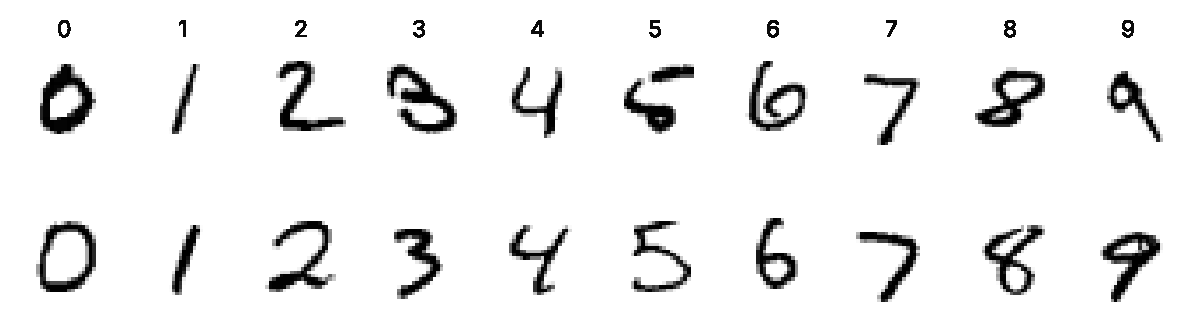
\includegraphics[width=0.92\linewidth]{fig_muestras_mnist.pdf}
  \caption{Dos ejemplos de cada dígito del conjunto de prueba de MNIST.}
  \label{fig:muestras}
\end{figure}

\subsection{Arquitectura utilizada}

Se implementó una CNN sencilla con dos bloques convolución--ReLU--\emph{max pooling} seguidos de un clasificador totalmente conectado con \emph{dropout} \parencite{srivastava2014} (Figura~\ref{fig:arquitectura} y Tabla~\ref{tab:arquitectura}).

\begin{figure}[H]
\centering
\resizebox{\linewidth}{!}{%
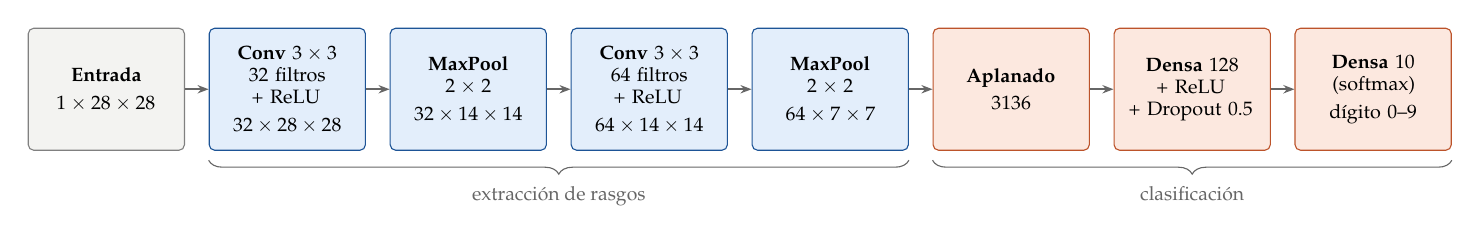
\begin{tikzpicture}[
  node distance=0.3cm,
  capa/.style={draw=azul!70!black, fill=azulclaro, rounded corners=2pt, align=center,
               minimum height=1.55cm, text width=1.75cm, font=\scriptsize},
  dens/.style={capa, draw=naranja!80!black, fill=naranjaclaro},
  ent/.style={capa, draw=black!50, fill=grisclaro},
  flecha/.style={-{Stealth[length=4pt]}, thick, black!60}]
  \node[ent]  (in) {\textbf{Entrada}\\[2pt]$1\times28\times28$};
  \node[capa, right=of in] (c1) {\textbf{Conv} $3\times3$\\32 filtros\\+ ReLU\\[2pt]$32\times28\times28$};
  \node[capa, right=of c1] (p1) {\textbf{MaxPool}\\$2\times2$\\[2pt]$32\times14\times14$};
  \node[capa, right=of p1] (c2) {\textbf{Conv} $3\times3$\\64 filtros\\+ ReLU\\[2pt]$64\times14\times14$};
  \node[capa, right=of c2] (p2) {\textbf{MaxPool}\\$2\times2$\\[2pt]$64\times7\times7$};
  \node[dens, right=of p2] (fl) {\textbf{Aplanado}\\[2pt]3136};
  \node[dens, right=of fl] (d1) {\textbf{Densa} 128\\+ ReLU\\+ Dropout 0.5};
  \node[dens, right=of d1] (d2) {\textbf{Densa} 10\\(softmax)\\[2pt]dígito 0--9};
  \foreach \a/\b in {in/c1,c1/p1,p1/c2,c2/p2,p2/fl,fl/d1,d1/d2}
    \draw[flecha] (\a) -- (\b);
  \draw[decorate,decoration={brace,amplitude=5pt,mirror},black!60]
    ($(c1.south west)+(0,-0.12)$) -- ($(p2.south east)+(0,-0.12)$)
    node[midway,below=6pt,font=\scriptsize\color{gris}]{extracción de rasgos};
  \draw[decorate,decoration={brace,amplitude=5pt,mirror},black!60]
    ($(fl.south west)+(0,-0.12)$) -- ($(d2.south east)+(0,-0.12)$)
    node[midway,below=6pt,font=\scriptsize\color{gris}]{clasificación};
\end{tikzpicture}}
\caption{Arquitectura de la CNN implementada. Debajo de cada capa se indica la forma de su salida (canales $\times$ alto $\times$ ancho).}
\label{fig:arquitectura}
\end{figure}

\begin{table}[H]
\centering
\caption{Capas, forma de la salida y número de parámetros de la CNN.}
\label{tab:arquitectura}
\small
\setlength{\tabcolsep}{5pt}
\begin{tabular}{llllr}
\toprule
\textbf{Capa} & \textbf{Configuración} & \textbf{Salida} & \textbf{Cálculo de parámetros} & \textbf{Parámetros} \\
\midrule
Conv2d 1     & 32 filtros $3\times3$, relleno 1 & $32\times28\times28$ & $(3\cdot3\cdot1+1)\cdot32$   & 320 \\
ReLU + MaxPool & ventana $2\times2$, paso 2          & $32\times14\times14$ & --                           & 0 \\
Conv2d 2     & 64 filtros $3\times3$, relleno 1 & $64\times14\times14$ & $(3\cdot3\cdot32+1)\cdot64$  & 18{,}496 \\
ReLU + MaxPool & ventana $2\times2$, paso 2          & $64\times7\times7$   & --                           & 0 \\
Aplanado     & --                                      & 3136                 & --                           & 0 \\
Densa 1      & 128 + ReLU + Dropout 0.5 & 128                  & $3136\cdot128+128$           & 401{,}536 \\
Densa 2      & 10 (logits) & 10                   & $128\cdot10+10$              & 1{,}290 \\
\midrule
\multicolumn{4}{l}{\textbf{Número total de parámetros (todos entrenables)}} & \textbf{\ParamTotal} \\
\bottomrule
\end{tabular}
\end{table}

La red tiene \textbf{\ParamTotal{} parámetros}, de los cuales el 95\pct{} está en la primera capa densa. La definición en PyTorch es:

\begin{lstlisting}
class CNNSencilla(nn.Module):
    def __init__(self, num_clases=10):
        super().__init__()
        self.bloque1 = nn.Sequential(                    # 1x28x28 -> 32x14x14
            nn.Conv2d(1, 32, kernel_size=3, padding=1), nn.ReLU(), nn.MaxPool2d(2))
        self.bloque2 = nn.Sequential(                    # 32x14x14 -> 64x7x7
            nn.Conv2d(32, 64, kernel_size=3, padding=1), nn.ReLU(), nn.MaxPool2d(2))
        self.clasificador = nn.Sequential(               # 3136 -> 128 -> 10
            nn.Flatten(), nn.Linear(64 * 7 * 7, 128), nn.ReLU(),
            nn.Dropout(p=0.5), nn.Linear(128, num_clases))

    def forward(self, x):
        return self.clasificador(self.bloque2(self.bloque1(x)))   # logits
\end{lstlisting}

\subsection{Entrenamiento}

El modelo se entrenó durante \Epocas{} épocas con el optimizador Adam \parencite{adam} (tasa de aprendizaje $10^{-3}$), lotes de \TamLote{} imágenes y la función de pérdida de entropía cruzada. El entrenamiento se ejecutó en CPU (2 hilos) y tardó \TiempoEnt{}~s en total (unos \TiempoEpoca{}~s por época). La Figura~\ref{fig:curvas} y la Tabla~\ref{tab:historial} muestran la evolución por época.

\begin{figure}[H]
  \centering
  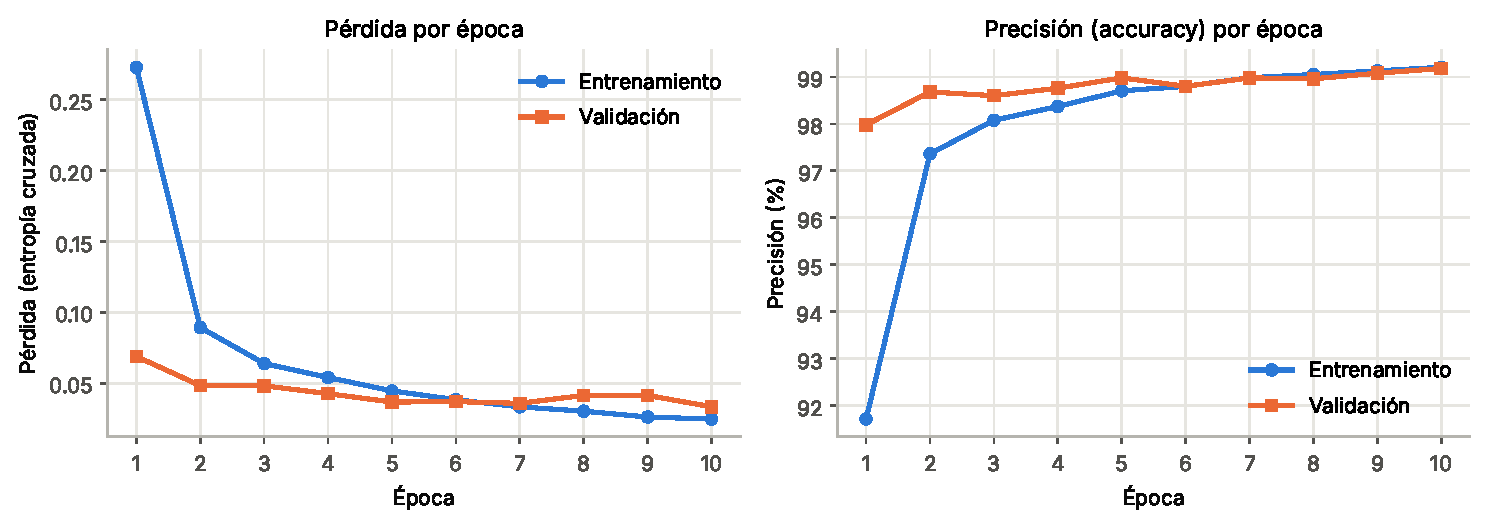
\includegraphics[width=\linewidth]{fig_curvas_entrenamiento.pdf}
  \caption{Pérdida y exactitud por época en entrenamiento (promedio durante la época, con \emph{dropout} activo) y en validación.}
  \label{fig:curvas}
\end{figure}

\begin{table}[H]
\centering
\caption{Historial de entrenamiento. Las métricas de entrenamiento son el promedio durante cada época (con \emph{dropout} activo).}
\label{tab:historial}
\small
\begin{tabular}{cccccc}
\toprule
\textbf{Época} & \textbf{Pérdida ent.} & \textbf{Exactitud ent. (\%)} & \textbf{Pérdida val.} & \textbf{Exactitud val. (\%)} & \textbf{Tiempo (s)} \\
\midrule
\FilasHistorial
\bottomrule
\end{tabular}
\end{table}

En las primeras épocas la exactitud de validación es \emph{mayor} que la de entrenamiento. No es un error: la métrica de entrenamiento se promedia mientras los pesos aún están cambiando y con \emph{dropout} activo (la mitad de las neuronas densas apagadas), mientras que la validación se mide al final de la época con la red completa.

\subsection{Resultados}

Al terminar el entrenamiento, el modelo se evaluó en modo de evaluación (sin \emph{dropout}) sobre los tres conjuntos (Tabla~\ref{tab:resultados}).

\begin{table}[H]
\centering
\caption{Desempeño final de la CNN.}
\label{tab:resultados}
\begin{tabular}{lccc}
\toprule
\textbf{Conjunto} & \textbf{Imágenes} & \textbf{Exactitud (\%)} & \textbf{Pérdida} \\
\midrule
Entrenamiento & 55{,}000 & \textbf{\AccTrain} & \LossTrain \\
Validación    & 5{,}000  & \AccVal & \LossVal \\
Prueba        & 10{,}000 & \textbf{\AccTest} & \LossTest \\
\bottomrule
\end{tabular}
\end{table}

\begin{itemize}
  \item \textbf{Precisión (exactitud) de entrenamiento: \AccTrain\pct{}.}
  \item \textbf{Precisión (exactitud) de prueba: \AccTest\pct{}}, es decir, \NErroresTest{} errores en 10{,}000 imágenes (tasa de error de \ErrTest\pct{}).
\end{itemize}

\paragraph{Matriz de confusión.} La Figura~\ref{fig:confusion} muestra la matriz de confusión del conjunto de prueba. La diagonal concentra los aciertos; los valores fuera de ella son los errores. Se usó una escala de color logarítmica para que los errores, que son pocos, también se distingan.

\begin{figure}[H]
  \centering
  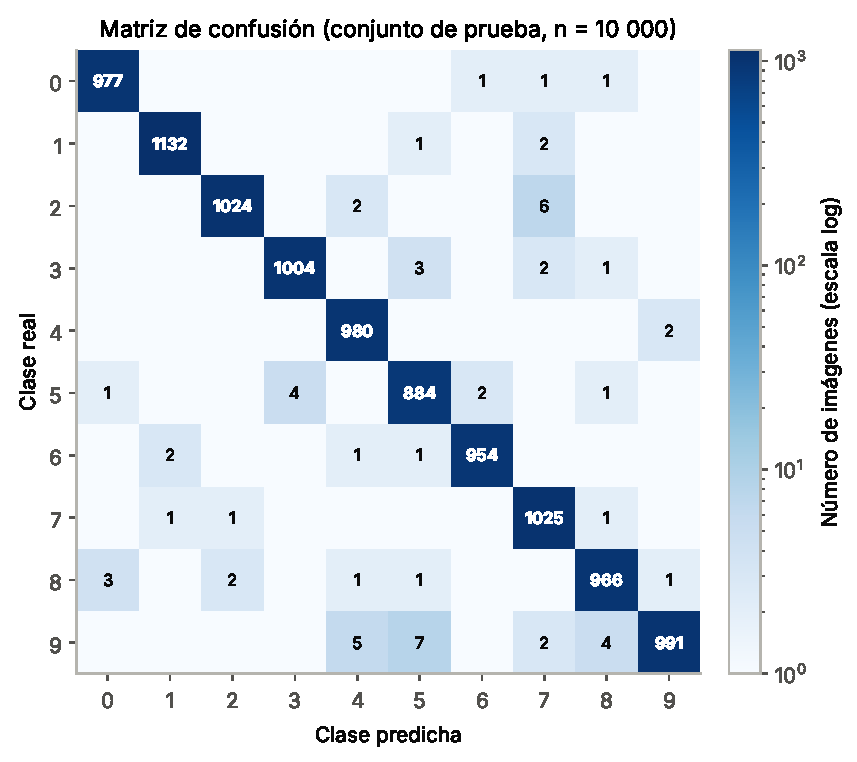
\includegraphics[width=0.66\linewidth]{fig_matriz_confusion.pdf}
  \caption{Matriz de confusión del conjunto de prueba (filas: clase real; columnas: clase predicha).}
  \label{fig:confusion}
\end{figure}

\paragraph{Métricas por clase.} La Tabla~\ref{tab:porclase} reporta la precisión, la exhaustividad y F1 de cada dígito (definidas en la Sección~\ref{sec:metricas}).

\begin{table}[H]
\centering
\caption{Métricas por clase en el conjunto de prueba.}
\label{tab:porclase}
\small
\begin{tabular}{ccccc}
\toprule
\textbf{Dígito} & \textbf{Precisión (\%)} & \textbf{Exhaustividad (\%)} & \textbf{F1 (\%)} & \textbf{Imágenes} \\
\midrule
\FilasPorClase
\midrule
\textbf{Promedio macro} & \MacroP & \MacroR & \MacroF & 10{,}000 \\
\bottomrule
\end{tabular}
\end{table}

\subsection{Ejemplos clasificados correcta e incorrectamente}

La Figura~\ref{fig:correctos} muestra cinco imágenes de prueba clasificadas correctamente (elegidas al azar, de dígitos distintos) y la Figura~\ref{fig:incorrectos}, cinco clasificadas incorrectamente. Para estas últimas se eligieron los cinco errores en los que el modelo estaba \emph{más seguro} de su respuesta, porque son los más informativos. Sobre cada imagen se indica la clase real, la predicha, la probabilidad que el modelo asignó a su predicción y el índice de la imagen en el conjunto de prueba.

\begin{figure}[H]
  \centering
  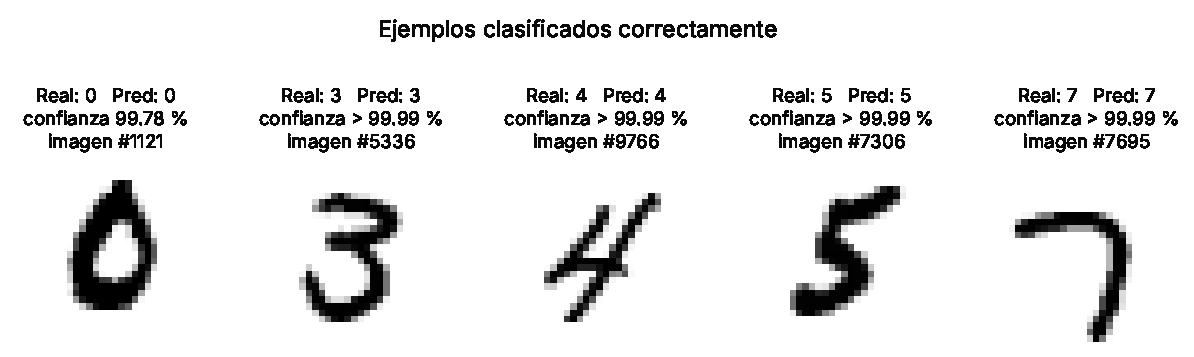
\includegraphics[width=0.95\linewidth]{fig_ejemplos_correctos.pdf}
  \caption{Cinco ejemplos clasificados correctamente.}
  \label{fig:correctos}
\end{figure}

\begin{figure}[H]
  \centering
  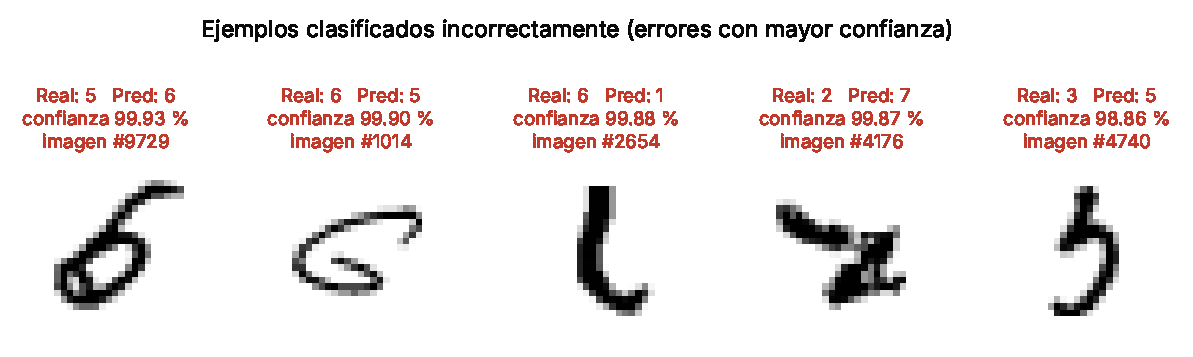
\includegraphics[width=0.95\linewidth]{fig_ejemplos_incorrectos.pdf}
  \caption{Cinco ejemplos clasificados incorrectamente (los errores con mayor confianza).}
  \label{fig:incorrectos}
\end{figure}

Los aciertos corresponden a trazos claros y típicos de cada dígito, que el modelo reconoce con una confianza prácticamente total. Los errores, en cambio, son imágenes atípicas o ambiguas incluso para una persona: un 5 cuyo trazo inferior se cierra en un lazo y se parece a un 6 (\#\ErrAIdx); un 6 muy inclinado y abierto que recuerda a un 5 (\#\ErrBIdx); un 6 sin lazo inferior que parece un 1 (\#\ErrCIdx); un 2 con trazo grueso e irregular que se confunde con un 7 (\#\ErrDIdx) y un 3 con la parte superior plana, parecido a un 5 (\#\ErrEIdx).

\subsection{Análisis de resultados}

\begin{itemize}
  \item \textbf{Buen desempeño y poco sobreajuste.} Con solo dos capas convolucionales y \TiempoEntMin{} minutos de entrenamiento en CPU, la red clasificó correctamente \NAciertosTest{} de 10{,}000 imágenes de prueba (\AccTest\pct{}). La diferencia entre la exactitud de entrenamiento (\AccTrain\pct{}) y la de prueba (\AccTest\pct{}) es menor a medio punto porcentual, lo que indica que el modelo generaliza bien; el \emph{dropout} contribuye a ello. Como referencia histórica, LeNet-5 reportó 0.95\pct{} de error en este mismo conjunto \parencite{lecun1998}; nuestra red obtiene \ErrTest\pct{}.
  \item \textbf{Curvas de aprendizaje.} La pérdida de validación baja rápido durante las primeras épocas y después se estabiliza alrededor de 0.035--0.04, con pequeñas oscilaciones (épocas 8 y 9), mientras que la de entrenamiento sigue bajando. Esto indica que el modelo está cerca de su capacidad máxima con esta configuración y que entrenar muchas más épocas, con la misma tasa de aprendizaje, empezaría a producir sobreajuste.
  \item \textbf{Errores concentrados en dígitos de forma parecida.} El dígito con menor F1 es el \PeorClase{} (\PeorClaseF\pct{}), y el 9 tiene la menor exhaustividad (\ErroresNueve{} de sus imágenes se clasificaron mal). Los pares más confundidos son \ParA{} (\ParAN{} casos), \ParB{} (\ParBN), \ParC{} (\ParCN), \ParD{} (\ParDN) y \ParE{} (\ParEN): dígitos que comparten trazos. El 9 tiene un lazo superior y un trazo descendente; si el lazo queda abierto o anguloso se parece a un 4 o a un 5, y si el trazo inferior se curva, a un 8. El 2 y el 7 comparten la diagonal larga, y el 3 y el 5, la curva inferior. El mejor reconocido es el \MejorClase{} (F1 de \MejorClaseF\pct{}).
  \item \textbf{Exceso de confianza.} En los errores de la Figura~\ref{fig:incorrectos} el modelo asignó más de 98\pct{} de probabilidad a la clase equivocada. Las redes modernas tienden a estar mal \emph{calibradas}: su probabilidad de salida no refleja la probabilidad real de acertar \parencite{guo2017}. En una aplicación real (por ejemplo, lectura de cheques) convendría calibrar el modelo para poder enviar a revisión humana las imágenes dudosas.
\end{itemize}

\subsubsection{Comparación con métodos clásicos}
\label{sec:clasicos}

Para conectar estos resultados con la Parte~II, se entrenaron dos métodos clásicos con exactamente las mismas 55{,}000 imágenes de entrenamiento y se evaluaron en las mismas 10{,}000 de prueba (Tabla~\ref{tab:clasicos}): $k$ vecinos más cercanos \parencite{cover1967} sobre los píxeles crudos, y el descriptor HOG \parencite{dalal2005} (celdas de $7\times7$, bloques de $2\times2$, 9 orientaciones; \HogDim{} valores por imagen) con una SVM lineal \parencite{cortes1995}.

\begin{table}[H]
\centering
\caption{CNN frente a métodos clásicos en MNIST (mismos datos de entrenamiento y prueba, CPU de 2 hilos).}
\label{tab:clasicos}
\small
\begin{tabular}{lccccc}
\toprule
\textbf{Método} & \makecell{\textbf{Exactitud}\\\textbf{(\%)}} & \makecell{\textbf{Errores}\\\textbf{(de 10{,}000)}} & \makecell{\textbf{Parámetros}\\\textbf{aprendidos}} & \makecell{\textbf{Entrenamiento}\\\textbf{(s)}} & \makecell{\textbf{Predicción de}\\\textbf{10{,}000 imágenes (s)}} \\
\midrule
$k$-NN ($k=3$), píxeles & \KnnAcc & \KnnErrores & --\textsuperscript{a} & \KnnAjuste & \KnnPred \\
HOG + SVM lineal        & \HogAcc & \HogErrores & \HogParam & \HogExtr{} + \HogAjuste\textsuperscript{b} & \HogPred \\
\textbf{CNN (este trabajo)} & \textbf{\AccTest} & \textbf{\NErroresTest} & \ParamTotal & \TiempoEnt & \TiempoInf \\
\bottomrule
\multicolumn{6}{l}{\footnotesize \textsuperscript{a} $k$-NN no aprende parámetros: almacena las 55{,}000 imágenes y las compara con cada imagen nueva.}\\
\multicolumn{6}{l}{\footnotesize \textsuperscript{b} Extracción de HOG + ajuste de la SVM.}
\end{tabular}
\end{table}

La CNN comete entre cuatro y cinco veces menos errores que los métodos clásicos, a cambio de unas 130 veces más parámetros que la SVM y un entrenamiento varias veces más largo. Aun así, los métodos clásicos superan el 96\pct{} sin aprender ningún rasgo, lo que ilustra la conclusión de la Parte~II: cuando los recursos son limitados o se necesita un modelo simple e interpretable, siguen siendo una opción razonable.

\subsection{Mejoras propuestas}

\begin{enumerate}
  \item \textbf{Aumento de datos} (\emph{data augmentation}). Los errores observados se deben sobre todo a la variabilidad de la escritura: inclinación, grosor del trazo, lazos abiertos o cerrados. Aplicar durante el entrenamiento transformaciones aleatorias pequeñas (rotaciones de $\pm10^\circ$, traslaciones de 2--3 píxeles, cambios de escala y deformaciones elásticas) expone a la red a más variantes de cada dígito sin etiquetar imágenes nuevas. \textcite{simard2003} mostraron que las distorsiones elásticas reducen notablemente el error de una CNN sencilla en MNIST. En PyTorch basta con añadir \texttt{transforms.RandomAffine} (o \texttt{transforms.ElasticTransform}) a la transformación de entrenamiento.
  \item \textbf{Red un poco más profunda con normalización por lotes y ajuste de la tasa de aprendizaje.} Usar dos convoluciones por bloque (y un tercer bloque), cada una seguida de \emph{batch normalization} \parencite{ioffe2015}, y sustituir el aplanado más la gran capa densa por \emph{global average pooling}. Esto aumenta la capacidad de extraer rasgos y, a la vez, reduce los parámetros (hoy, el 95\pct{} está en la primera capa densa). Además, reducir la tasa de aprendizaje cuando la pérdida de validación deja de mejorar (\texttt{ReduceLROnPlateau}) o con un programa de tipo coseno estabilizaría las oscilaciones de las últimas épocas, y detener el entrenamiento en la mejor época de validación (\emph{early stopping}) evitaría el sobreajuste.
\end{enumerate}

\section*{Conclusiones generales}
\addcontentsline{toc}{section}{Conclusiones generales}

Las redes neuronales convolucionales cambiaron el procesamiento de imágenes porque aprenden directamente de los datos los filtros que antes se diseñaban a mano, y arquitecturas como ResNet, EfficientNet, U-Net y ViT extendieron esa idea a redes más profundas, más eficientes, a la segmentación y a los mecanismos de atención. Nuestra implementación lo confirma a pequeña escala: una CNN de \ParamTotal{} parámetros alcanzó \AccTest\pct{} de exactitud en MNIST tras \TiempoEntMin{} minutos de entrenamiento en CPU, superando claramente a $k$-NN y a HOG con SVM. Sin embargo, la comparación también mostró el valor vigente de los métodos clásicos: con muy pocos parámetros y sin aprender rasgos, superan el 96\pct{}, y son más interpretables y baratos. La IA es la mejor herramienta cuando hay datos y cómputo suficientes y el problema es muy variable; los métodos clásicos siguen siendo la opción adecuada en problemas acotados, con pocos datos, hardware limitado o necesidad de explicar cada decisión, y lo más común en la práctica es combinarlos.

% =============================================================================
\clearpage
\section*{Referencias}
\addcontentsline{toc}{section}{Referencias}
\begingroup
\small
\setlength{\parindent}{-1.27cm}
\setlength{\leftskip}{1.27cm}
\setlength{\parskip}{5pt}
\raggedright

Cortes, C., \& Vapnik, V. (1995). Support-vector networks. \emph{Machine Learning, 20}(3), 273--297. \url{https://doi.org/10.1007/BF00994018}

Cover, T., \& Hart, P. (1967). Nearest neighbor pattern classification. \emph{IEEE Transactions on Information Theory, 13}(1), 21--27. \url{https://doi.org/10.1109/TIT.1967.1053964}

Dalal, N., \& Triggs, B. (2005). Histograms of oriented gradients for human detection. En \emph{2005 IEEE Computer Society Conference on Computer Vision and Pattern Recognition (CVPR'05)} (Vol. 1, pp. 886--893). IEEE. \url{https://doi.org/10.1109/CVPR.2005.177}

Deng, J., Dong, W., Socher, R., Li, L.-J., Li, K., \& Fei-Fei, L. (2009). ImageNet: A large-scale hierarchical image database. En \emph{2009 IEEE Conference on Computer Vision and Pattern Recognition} (pp. 248--255). IEEE. \url{https://doi.org/10.1109/CVPR.2009.5206848}

Dosovitskiy, A., Beyer, L., Kolesnikov, A., Weissenborn, D., Zhai, X., Unterthiner, T., Dehghani, M., Minderer, M., Heigold, G., Gelly, S., Uszkoreit, J., \& Houlsby, N. (2021). An image is worth 16x16 words: Transformers for image recognition at scale. En \emph{International Conference on Learning Representations (ICLR 2021)}. \url{https://openreview.net/forum?id=YicbFdNTTy}

Freeman, H. (1961). On the encoding of arbitrary geometric configurations. \emph{IRE Transactions on Electronic Computers, EC-10}(2), 260--268. \url{https://doi.org/10.1109/TEC.1961.5219197}

Gonzalez, R. C., \& Woods, R. E. (2018). \emph{Digital image processing} (4.ª ed.). Pearson.

Goodfellow, I., Bengio, Y., \& Courville, A. (2016). \emph{Deep learning}. MIT Press. \url{https://www.deeplearningbook.org}

Guo, C., Pleiss, G., Sun, Y., \& Weinberger, K. Q. (2017). On calibration of modern neural networks. En \emph{Proceedings of the 34th International Conference on Machine Learning} (Vol. 70, pp. 1321--1330). PMLR.

He, K., Zhang, X., Ren, S., \& Sun, J. (2016). Deep residual learning for image recognition. En \emph{Proceedings of the IEEE Conference on Computer Vision and Pattern Recognition (CVPR)} (pp. 770--778). \url{https://doi.org/10.1109/CVPR.2016.90}

Ioffe, S., \& Szegedy, C. (2015). Batch normalization: Accelerating deep network training by reducing internal covariate shift. En \emph{Proceedings of the 32nd International Conference on Machine Learning} (Vol. 37, pp. 448--456). PMLR.

Kingma, D. P., \& Ba, J. (2015). Adam: A method for stochastic optimization. En \emph{3rd International Conference on Learning Representations (ICLR 2015)}. \url{https://arxiv.org/abs/1412.6980}

LeCun, Y., Bottou, L., Bengio, Y., \& Haffner, P. (1998). Gradient-based learning applied to document recognition. \emph{Proceedings of the IEEE, 86}(11), 2278--2324. \url{https://doi.org/10.1109/5.726791}

LeCun, Y., Cortes, C., \& Burges, C. J. C. (1998). \emph{The MNIST database of handwritten digits} [Conjunto de datos]. \url{http://yann.lecun.com/exdb/mnist/}

Lowe, D. G. (2004). Distinctive image features from scale-invariant keypoints. \emph{International Journal of Computer Vision, 60}(2), 91--110. \url{https://doi.org/10.1023/B:VISI.0000029664.99615.94}

Nair, V., \& Hinton, G. E. (2010). Rectified linear units improve restricted Boltzmann machines. En \emph{Proceedings of the 27th International Conference on Machine Learning (ICML-10)} (pp. 807--814).

O'Mahony, N., Campbell, S., Carvalho, A., Harapanahalli, S., Velasco Hernandez, G., Krpalkova, L., Riordan, D., \& Walsh, J. (2020). Deep learning vs. traditional computer vision. En K. Arai \& S. Kapoor (Eds.), \emph{Advances in computer vision: Proceedings of the 2019 Computer Vision Conference (CVC)} (Advances in Intelligent Systems and Computing, Vol. 943, pp. 128--144). Springer. \url{https://doi.org/10.1007/978-3-030-17795-9_10}

Pan, S. J., \& Yang, Q. (2010). A survey on transfer learning. \emph{IEEE Transactions on Knowledge and Data Engineering, 22}(10), 1345--1359. \url{https://doi.org/10.1109/TKDE.2009.191}

Paszke, A., Gross, S., Massa, F., Lerer, A., Bradbury, J., Chanan, G., Killeen, T., Lin, Z., Gimelshein, N., Antiga, L., Desmaison, A., Köpf, A., Yang, E., DeVito, Z., Raison, M., Tejani, A., Chilamkurthy, S., Steiner, B., Fang, L., \ldots{} Chintala, S. (2019). PyTorch: An imperative style, high-performance deep learning library. En \emph{Advances in Neural Information Processing Systems 32} (pp. 8024--8035).

Pedregosa, F., Varoquaux, G., Gramfort, A., Michel, V., Thirion, B., Grisel, O., Blondel, M., Prettenhofer, P., Weiss, R., Dubourg, V., Vanderplas, J., Passos, A., Cournapeau, D., Brucher, M., Perrot, M., \& Duchesnay, É. (2011). Scikit-learn: Machine learning in Python. \emph{Journal of Machine Learning Research, 12}, 2825--2830.

Ronneberger, O., Fischer, P., \& Brox, T. (2015). U-Net: Convolutional networks for biomedical image segmentation. En N. Navab, J. Hornegger, W. M. Wells, \& A. F. Frangi (Eds.), \emph{Medical Image Computing and Computer-Assisted Intervention -- MICCAI 2015} (Lecture Notes in Computer Science, Vol. 9351, pp. 234--241). Springer. \url{https://doi.org/10.1007/978-3-319-24574-4_28}

Rosenblatt, F. (1958). The perceptron: A probabilistic model for information storage and organization in the brain. \emph{Psychological Review, 65}(6), 386--408. \url{https://doi.org/10.1037/h0042519}

Rumelhart, D. E., Hinton, G. E., \& Williams, R. J. (1986). Learning representations by back-propagating errors. \emph{Nature, 323}(6088), 533--536. \url{https://doi.org/10.1038/323533a0}

Selvaraju, R. R., Cogswell, M., Das, A., Vedantam, R., Parikh, D., \& Batra, D. (2017). Grad-CAM: Visual explanations from deep networks via gradient-based localization. En \emph{Proceedings of the IEEE International Conference on Computer Vision (ICCV)} (pp. 618--626). \url{https://doi.org/10.1109/ICCV.2017.74}

Simard, P. Y., Steinkraus, D., \& Platt, J. C. (2003). Best practices for convolutional neural networks applied to visual document analysis. En \emph{Proceedings of the Seventh International Conference on Document Analysis and Recognition (ICDAR 2003)} (pp. 958--962). IEEE. \url{https://doi.org/10.1109/ICDAR.2003.1227801}

Sokolova, M., \& Lapalme, G. (2009). A systematic analysis of performance measures for classification tasks. \emph{Information Processing \& Management, 45}(4), 427--437. \url{https://doi.org/10.1016/j.ipm.2009.03.002}

Srivastava, N., Hinton, G., Krizhevsky, A., Sutskever, I., \& Salakhutdinov, R. (2014). Dropout: A simple way to prevent neural networks from overfitting. \emph{Journal of Machine Learning Research, 15}(56), 1929--1958.

Szeliski, R. (2022). \emph{Computer vision: Algorithms and applications} (2.ª ed.). Springer. \url{https://doi.org/10.1007/978-3-030-34372-9}

Tan, M., \& Le, Q. (2019). EfficientNet: Rethinking model scaling for convolutional neural networks. En K. Chaudhuri \& R. Salakhutdinov (Eds.), \emph{Proceedings of the 36th International Conference on Machine Learning} (Vol. 97, pp. 6105--6114). PMLR.

Vaswani, A., Shazeer, N., Parmar, N., Uszkoreit, J., Jones, L., Gomez, A. N., Kaiser, Ł., \& Polosukhin, I. (2017). Attention is all you need. En \emph{Advances in Neural Information Processing Systems 30} (pp. 5998--6008).

Yosinski, J., Clune, J., Bengio, Y., \& Lipson, H. (2014). How transferable are features in deep neural networks? En \emph{Advances in Neural Information Processing Systems 27} (pp. 3320--3328).

\endgroup
\end{document}
